In this section we illustrate the possibilities of our description
language.  The first system studied is a distributed database system.
Then we describe a load balancing system which makes use of more
advanced features of our tool.  The third example is the well-known
puzzle of the towers of Hanoi.  This one illustrates a use of
high-level data types provided by Helena.

\section{The distributed database system}We consider in this system a set of $N$ database managers which
communicate to maintain consistent replica of a database.  It is a
well-known and recurrent example of the colored Petri nets literature,
initially presented by Genrich and later by Jensen.

When a manager updates its local copy of the database, he sends
requests to other managers for updating their local copy (transition
{\it Update}). As soon as a manager receives such a request
(transition {\it Receive}) he starts the update of its copy. Its
update finished, each manager acknowledges the initiating manager
(transition {\it Send ack}).  This process finishes when the
initiating manager collects all the acknowledgments (transition {\it
Receive acks}). Managers can be either {\it Inactive}, either {\it
Waiting} for acknowledgments, either {\it Performing} an
update. Places {\it Msgs}, {\it Received}, {\it Acks} and {\it Unused}
model communication channels between sites. Thus, $N.(N-1)$ tokens are
distributed upon these places at each marking. At last the correctness
of the protocol is ensured by place \lstinline{Mutex} which guarantees
that two managers cannot concurrently update their local copy.

\begin{figure}[!h]
\centerline{\scalebox{0.55}{We consider in this system a set of $N$ database managers which
communicate to maintain consistent replica of a database.  It is a
well-known and recurrent example of the colored Petri nets literature,
initially presented by Genrich and later by Jensen.

When a manager updates its local copy of the database, he sends
requests to other managers for updating their local copy (transition
{\it Update}). As soon as a manager receives such a request
(transition {\it Receive}) he starts the update of its copy. Its
update finished, each manager acknowledges the initiating manager
(transition {\it Send ack}).  This process finishes when the
initiating manager collects all the acknowledgments (transition {\it
Receive acks}). Managers can be either {\it Inactive}, either {\it
Waiting} for acknowledgments, either {\it Performing} an
update. Places {\it Msgs}, {\it Received}, {\it Acks} and {\it Unused}
model communication channels between sites. Thus, $N.(N-1)$ tokens are
distributed upon these places at each marking. At last the correctness
of the protocol is ensured by place \lstinline{Mutex} which guarantees
that two managers cannot concurrently update their local copy.

\begin{figure}[!h]
\centerline{\scalebox{0.55}{We consider in this system a set of $N$ database managers which
communicate to maintain consistent replica of a database.  It is a
well-known and recurrent example of the colored Petri nets literature,
initially presented by Genrich and later by Jensen.

When a manager updates its local copy of the database, he sends
requests to other managers for updating their local copy (transition
{\it Update}). As soon as a manager receives such a request
(transition {\it Receive}) he starts the update of its copy. Its
update finished, each manager acknowledges the initiating manager
(transition {\it Send ack}).  This process finishes when the
initiating manager collects all the acknowledgments (transition {\it
Receive acks}). Managers can be either {\it Inactive}, either {\it
Waiting} for acknowledgments, either {\it Performing} an
update. Places {\it Msgs}, {\it Received}, {\it Acks} and {\it Unused}
model communication channels between sites. Thus, $N.(N-1)$ tokens are
distributed upon these places at each marking. At last the correctness
of the protocol is ensured by place \lstinline{Mutex} which guarantees
that two managers cannot concurrently update their local copy.

\begin{figure}[!h]
\centerline{\scalebox{0.55}{\input{dbm.pdf_t}}}
\caption{The distributed database system}
\label{fig_dbm}
\end{figure}

\lstinputlisting[frame=single,
caption={Helena file of the distributed database system
(file \texttt{examples/dbm.lna})},
numbers=left,basicstyle=\small] {../examples/dbm.lna}

\lstinputlisting[frame=single,
caption={Helena file of the distributed database system properties
(file \texttt{examples/dbm.prop.lna})},
numbers=left,basicstyle=\small] {../examples/dbm.prop.lna}
}}
\caption{The distributed database system}
\label{fig_dbm}
\end{figure}

\lstinputlisting[frame=single,
caption={Helena file of the distributed database system
(file \texttt{examples/dbm.lna})},
numbers=left,basicstyle=\small] {../examples/dbm.lna}

\lstinputlisting[frame=single,
caption={Helena file of the distributed database system properties
(file \texttt{examples/dbm.prop.lna})},
numbers=left,basicstyle=\small] {../examples/dbm.prop.lna}
}}
\caption{The distributed database system}
\label{fig_dbm}
\end{figure}

\lstinputlisting[frame=single,
caption={Helena file of the distributed database system
(file \texttt{examples/dbm.lna})},
numbers=left,basicstyle=\small] {../examples/dbm.lna}

\lstinputlisting[frame=single,
caption={Helena file of the distributed database system properties
(file \texttt{examples/dbm.prop.lna})},
numbers=left,basicstyle=\small] {../examples/dbm.prop.lna}

\section{The load balancing system}We propose to specify and verify a simple load balancing system with
Helena.  The full net is illustrated by
Figure~\ref{fig_load_balancer}. Initial markings and transition guards
have been omitted to clarify the figure.

\begin{figure}[!h]
\centerline{\scalebox{0.5}{ 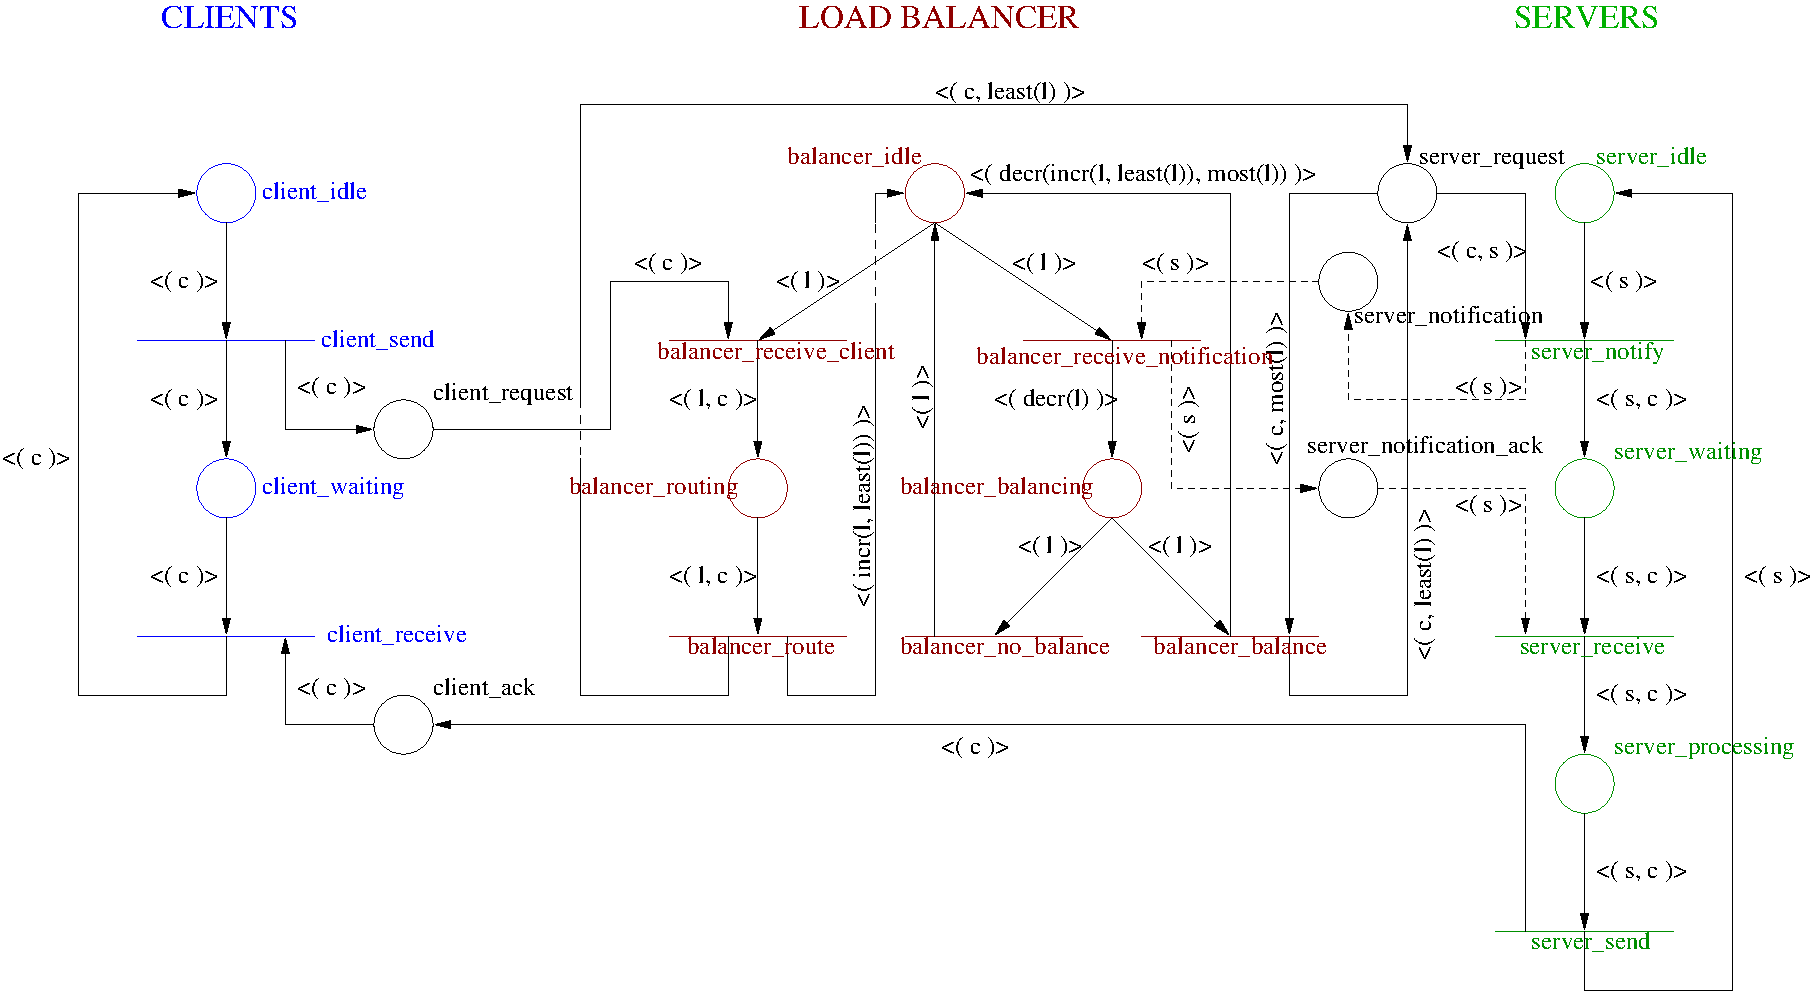
\includegraphics{load_balancer}}}
\caption{The whole load balancing system}
\label{fig_load_balancer}
\end{figure}

In this system, we have two kinds of process: a set of clients and a
set of servers. An additional process called the load balancer
distribute requests of clients to servers. Its task is also to
redistribute pending requests when servers accept requests in order to
maintain the loads of servers balanced.

\paragraph{The clients}
We note \lstinline{C} the number of clients considered. Clients are
numbered from \lstinline{1} to \lstinline{C}. The behavior of the
clients is quite simple. A client may want to send a request to a set
of servers. Instead of asking a server directly, he sends the request
to the load balancer which will route the request to the adequate
server, i.e., the least loaded server. Once the request sent, the
client waits for the answer. When this one arrives, the client comes
back to the idle state.

\paragraph{The servers}
The number of servers is noted \lstinline{S}. Servers are numbered from
\lstinline{1} to \lstinline{S}. Servers receive requests from clients via the
load balancer process. When a server accepts a request, he first has
to notify this to the load balancer process, in order that this one
rebalances the pending requests. Then he has to wait for an
acknowledgment from the load balancer to start treating the request.
Once the request treated, he directly sends the answer to the
concerned client and goes back to the idle state.

\paragraph{The load balancer}
The load balancer can perform two kinds of task. The first one is to
redirect each client request to the least loaded server. Secondly,
when a server accepts a request from a client the load balancer has to
rebalance the pending requests. If these are already balanced, the
load balancer has nothing to perform and can come back to its idle
state (transition \lstinline{balancer_no_balance}). If the loads are
not balanced, the load balancer takes a pending request of the most
loaded server and redirects it to the least loaded server (transition
\lstinline{balancer_balance}).   The load balancer has to maintain for
each server the number of requests sent to this server.

\lstinputlisting[frame=single,
caption={Helena file of the load balancing system
(file \texttt{examples/load\_balancer.lna})},
numbers=left,basicstyle=\small] {../examples/load_balancer.lna}

\lstinputlisting[frame=single,
caption={Helena file of the load balancing system properties
(file \texttt{examples/load\_balancer.prop.lna})},
numbers=left,basicstyle=\small] {../examples/load_balancer.prop.lna}

\section{The towers of Hanoi}The towers of Hanoi is a well-known mathematical game\footnote{The
  description is taken
  from \url{http://en.wikipedia.org/wiki/Tower_of_Hanoi}.}.  It
  consists of three towers, and a number of disks of different sizes
  which can slide onto any tower.  The puzzle starts with the disks
  neatly stacked in order of size on one tower, smallest at the top,
  thus making a conical shape.

The objective of the game is to move the entire stack to another
tower, obeying the following rules:
\begin{itemize}
\item Only one disk may be moved at a time.
\item Each move consists of taking the upper disk from one of the
  towers and sliding it onto another tower, on top of the other disks
  that may already be present on that tower.
\item No disk may be placed on top of a smaller disk.
\end{itemize}

This example illustrates the use of lists in Helena.

\lstinputlisting[frame=single,
caption={Helena file of the towers of Hanoi
(file \texttt{examples/hanoi.lna})},
numbers=left,basicstyle=\small] {../examples/hanoi.lna}

\lstinputlisting[frame=single,
caption={Helena file of the towers of Hanoi properties
(file \texttt{examples/hanoi.prop.lna})},
numbers=left,basicstyle=\small] {../examples/hanoi.prop.lna}

